\documentclass{beamer}
\usetheme{CMU}

\usepackage{pgf,pgfarrows,pgfnodes,pgfautomata,pgfheaps,pgfshade}
\usepackage{amsmath,amssymb}
\usepackage[utf8]{inputenc}
\usepackage{colortbl}
\usepackage[english]{babel}
\usepackage{booktabs}
\usepackage{slpython}
\usepackage{underscore}

\author{Luís Pedro Coelho}
\institute{Programming for Scientists}

\graphicspath{{figures/}{figures/generated/}{images/}}

\newcommand*{\code}[1]{\textsl{#1}}


\title{File Parsing \& Regular Expressions}
\begin{document}
\frame{\maketitle}

\begin{frame}[fragile]
\frametitle{File Representions}
\begin{block}{What's a File?}
A sequence of bytes.

\bigskip
(and meta-data).
\note{This is very unixy. Files in Windows can have multiple streams}
\end{block}
\end{frame}

\begin{frame}[fragile]
\frametitle{File Format Examples: FASTA format}
\begin{verbatim}
> qqq
ACTTTGTTATATATACTATCTGTATTTTC
CTGGGTGAGAGAGTGGTTGAGAGGGGGAA
CCCCCAACCACATTTCCCCACACCCCCTG
ACTTTCCTATATGTCCATTTTTATAATC
> ppp
TTTTTGGTATCTATTTTCCACTCATTCTTTAT
TACCCCAGTCATCACAAAACACACACACAACC
ATTATCTCTAATATATAATTTTACCTTT
\end{verbatim}
\end{frame}

\begin{frame}[fragile]
\frametitle{Parsing FASTA}

\begin{python}
sequences = []
curseq = ''
for line in file('input.fsa'):
    if line[0] == '>':
        sequences.append(curseq)
    else:
        curseq += line.strip()
sequences.append(curseq)
\end{python}
\end{frame}

\begin{frame}[fragile]
\frametitle{File Format Examples (II): GenBank}

\begin{verbatim}
LOCUS       SCU49845     5028 bp    DNA             PLN       21-JUN-1999
DEFINITION  Saccharomyces cerevisiae TCP1-beta gene, partial cds, and Axl2p
            (AXL2) and Rev7p (REV7) genes, complete cds.
ACCESSION   U49845
VERSION     U49845.1  GI:1293613
KEYWORDS    .
SOURCE      Saccharomyces cerevisiae (baker's yeast)
  ORGANISM  Saccharomyces cerevisiae
            Eukaryota; Fungi; Ascomycota; Saccharomycotina; Saccharomycetes;
            Saccharomycetales; Saccharomycetaceae; Saccharomyces.
...
ORIGIN
        1 gatcctccat atacaacggt atctccacct caggtttaga tctcaacaac ggaaccattg
       61 ccgacatgag acagttaggt atcgtcgaga gttacaagct aaaacgagca gtagtcagct
      121 ctgcatctga agccgctgaa gttctactaa gggtggataa catcatccgt gcaagaccaa
      181 gaaccgccaa tagacaacat atgtaacata tttaggatat acctcgaaaa taataaaccg
      241 ccacactgtc attattataa ttagaaacag aacgcaaaaa ttatccacta tataattcaa
      301 agacgcgaaa aaaaaagaac aacgcgtcat agaacttttg gcaattcgcg tcacaaataa
      361 attttggcaa cttatgtttc ctcttcgagc agtactcgag ccctgtctca agaatgtaat
\end{verbatim}
\end{frame}

\begin{frame}[fragile]
\frametitle{Representing Text}
\begin{block}{ASCII}
\begin{itemize}
\item 65: A
\item 66: B
\item \ldots
\item 48: 0
\item 49: 1
\item \ldots
\item \ldots
\end{itemize}

127 code points taken.
\end{block}
\end{frame}

\begin{frame}[fragile]
\frametitle{Two File Format Classes}

\begin{itemize}
\item Text files
\item Non-text files (binary files)
\end{itemize}
\end{frame}

\begin{frame}[fragile]
\begin{center}
\begin{tabular}{lllll}
\toprule
Size & Hex Value & Value & Meaning\\
\midrule
2 & 42 4D  &"BM"  &Magic Number (66, 77)\\
4 & 46 00 00 00 & 70 Bytes & Size of Bitmap\\
2 & 00 00 & Unused & Application Specific\\
2 & 00 00 & Unused & Application Specific\\
4 & 36 00 00 00 & 54 bytes & The offset of data.\\
4 & 28 00 00 00 & 40 bytes & Size of header. \\
4 & 02 00 00 00 & 2 pixels & The width in pixels\\
4 & 02 00 00 00 & 2 pixels & The height in pixels\\
2 & 01 00 & 1 plane & Number of color planes.\\
2 & 18 00 & 24 bits & The bits/pixel.\\
4 & 00 00 00 00 & 0 & No compression used\\
4 & 10 00 00 00 & 16 bytes & The size of the raw BMP data\\
4 & 13 0B 00 00 & 2,835 pixels/m& The horizontal resolution\\
4 & 13 0B 00 00 & 2,835 pixels/m& The vertical resolution\\
4 & 00 00 00 00 & 0 & Number of colors in the palette\\
4 & 00 00 00 00 & 0 & Means all colors are important\\
\bottomrule
\end{tabular}
\end{center}
\end{frame}

\begin{frame}[fragile]
\begin{center}
\begin{tabular}{lllll}
\toprule
Size & Hex Value & Value & Meaning\\
\midrule
3 & 00 00 FF & 0 0 255 & Red, Pixel (0,1)\\
3 & FF FF FF & 255 255 255 &  White, Pixel (1,1)\\
2 & 00 00    & 0 & Padding for 4 bytes/row\\
3 & FF 00 00 & 255 0 0 & Blue, Pixel (0,0)\\
3 & 00 FF 00 & 0 255 0 & Green, Pixel (1,0)\\
2 & 00 00    & 0  & Padding for 4 bytes/row\\
\bottomrule
\end{tabular}
\end{center}


\begin{flushright}
(Wikipedia)
\end{flushright}

\end{frame}

\begin{frame}[fragile]
\frametitle{Bitmap}

\centering
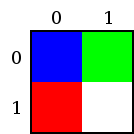
\includegraphics{BMPexample}

\end{frame}

\begin{frame}[fragile]
\frametitle{Text vs.\ Binary}
When possible, prefer text formats.

They are simpler.\note{but they still have a million quirks and we'll spend the rest of the lecture talking about them.}
\end{frame}

\begin{frame}[fragile]
\frametitle{Line Endings}
\begin{itemize}
\item Unix: LF (line feed)
\item Windows: CRLF (carriage return, line feed)
\item (Old Mac OS: CR)
\end{itemize}

The extra carriage returns will often show up as \^{}M in Unix.

Some unix text files will show up as a single ultra-long line on Windows.

\end{frame}


\begin{frame}[fragile]
\frametitle{What About International Characters?}

\begin{itemize}
\item Such as \'{a} or \c{c}?
\item Or $\mu$?
\item Or Asian characters?\note{I couldn't get asian characters in Latex, for example}
\item Or ---?

\end{itemize}
It's a mess!
\end{frame}

\begin{frame}[fragile]
\frametitle{International Character Sets}

\begin{itemize}
\item Traditional (latin-1,latin-9,latin-15,\ldots)
\item Unicode (16-bits, or 32-bits)
\item UTF-8
\end{itemize}
\end{frame}

\begin{frame}[fragile]
\frametitle{Unicode}

\begin{block}{Unicode}
Use 16~bits for (almost) all possible possible characters.\\
Use 32~bits for all possible characters.
\end{block}

\begin{block}{Byte Order}
If you have a 2~byte number, which byte do you write first?
\end{block}

\end{frame}

\begin{frame}[fragile]
\frametitle{UTF-8}
Emerging standard (at some levels).
\end{frame}

\note{break here}

\begin{frame}[fragile]
\frametitle{Parsing Files}
Let's say you had to parse the following ``file'':

\begin{verbatim}
Job id        Name          User     Time Use S Queue
----------- ------------- --------- -------- - -----
318695.c0-32 q1025-X.sh    jieyuel   169:29:2 R workq
320137.c0-32 q29199-X.sh   lcoelho   113:10:0 R workq
320139.c0-32 q29212-X.sh   lcoelho   113:29:0 R workq
320141.c0-32 q29226-X.sh   lcoelho   113:24:3 R workq
320143.c0-32 q29240-X.sh   lcoelho   113:09:3 R workq
320145.c0-32 q29254-X.sh   lcoelho   113:58:5 R workq
\end{verbatim}
\end{frame}

\begin{frame}[fragile]
\frametitle{First Try}

\begin{python}
for line in file('input.txt'):
    if line[0] not in '0123456789':
        continue
    jobid,name,user,time,s,queue = line.split()
    if user != 'lcoelho':
        continue
    jobid = jobid[:-len('.c0-32')] # 318695.c0-32
    runid = name[1:name.find('-')] # q1025-X.sh
    runid = int(runid)
    print "%-12s %-12s %-12%s' % (jobid,runid,time)

\end{python}
\end{frame}

\begin{frame}[fragile]
\frametitle{Regular Expressions}

\begin{itemize}
\item You have already seen regular expressions:
\verb+cat *.py+
\item A regular expression is a ``pattern''.
\end{itemize}

\note{Regular expressions are so important that some languages have built-in syntax for them (perl)}
\end{frame}

\begin{frame}[fragile]
\frametitle{Basic Regular Expressions}

\begin{itemize}
\item 'A', 'B', \ldots match themselves
\item '.' matches anything
\item '*' means repeat the previous any number of times\\
    (including zero)
\item '+' means repeat the previous at least once
\item '?' means one or zero of the previous
\item '[abc]' mean either 'a' or 'b' or 'c'
\item \ldots
\end{itemize}

\end{frame}


\begin{frame}[fragile]
\frametitle{Example}

\begin{python}
import re
line = '320143.c0-32 q29240-X.sh      lcoelho         113:09:3 R workq'
if re.match('[0-9]+.c0-32 q[0-9]+-X.sh +lcoelho +[0-9:]+.*',line):
    print 'matches!'
\end{python}

\end{frame}

\begin{frame}[fragile]
\frametitle{Get Information Out}
\begin{python}
import re
line = '320143.c0-32 q29240-X.sh      lcoelho         113:09:3 R workq'
match = re.match('([0-9]+).c0-32 q([0-9]+)-X.sh +lcoelho +([0-9:]+).*',line)
if match:
    jobid,runid,time = match.groups()
    print "%-12s %-12s %-12%s' % (jobid,runid,time)
\end{python}
\end{frame}

\begin{frame}[fragile]
\frametitle{Example}

Let's say your files look like this:
\begin{itemize}
\item experiment0\_t0\_0.txt
\item experiment0\_t0\_1.txt
\item experiment0\_t0\_2.txt
\item \ldots
\item experiment0\_t0\_14.txt
\item \ldots
\item experiment0\_t1\_0.txt
\item experiment0\_t1\_1.txt
\item \ldots
\item experiment1\_t0\_0.txt
\item \ldots
\item experiment123\_t124\_125.txt
\end{itemize}

You could match this with:

\begin{python}
import re
for file in os.listdir('.'):
    if re.match(r'experiment([0-9]+)_t([0-9]+)_([0-9]+)\.txt',line)
\end{python}

\end{frame}

\begin{frame}[fragile]
\frametitle{Compiling Patterns}
\begin{python}
import re
for file in os.listdir('.'):
    if re.match(r'experiment([0-9]+)_t([0-9]+)_([0-9]+)\.txt',line)
\end{python}
\begin{python}
import re
pat = re.compile(r'experiment([0-9]+)_t([0-9]+)_([0-9]+)\.txt')
for file in os.listdir('.'):
    if pat.match(line)
\end{python}
\end{frame}

\begin{frame}[fragile]
\frametitle{Closing Quote}

``Some people, when confronted with a problem, think \textit{I know, I’ll use regular expressions}. Now they have two problems.''

\end{frame}

\begin{frame}[fragile]
\frametitle{Example}

\begin{block}{Apache Log}
\begin{verbatim}

128.237.247.73 - - [17/Mar/2009:17:39:27 -0400] "GET /pfs/homeworks.html HTTP/1.1" 200 
        6997 "http://coupland.cbi.cmu.edu/pfs/" "Mozilla/4.0 (compatible; MSIE 7.0; 
        Windows NT 6.0; SLCC1; .NET CLR 2.0.50727; Media Center PC 5.0; .NET CLR 3.0.04506; InfoPath.2)"
128.237.247.73 - - [17/Mar/2009:17:39:42 -0400] "GET /pfs/index.html HTTP/1.1" 304 
        - "http://coupland.cbi.cmu.edu/pfs/homeworks.html" "Mozilla/4.0 (compatible; 
        MSIE 7.0; Windows NT 6.0; SLCC1; .NET CLR 2.0.50727; Media Center PC 5.0; .NET CLR 3.0.04506; InfoPath.2)"
128.237.247.73 - - [17/Mar/2009:17:39:45 -0400] "GET /pfs/project.html HTTP/1.1" 200
        4998 "http://coupland.cbi.cmu.edu/pfs/index.html" "Mozilla/4.0 (compatible; 
        MSIE 7.0; Windows NT 6.0; SLCC1; .NET CLR 2.0.50727; Media Center PC 5.0; .NET CLR 3.0.04506;InfoPath.2)"
\end{verbatim}
\end{block}
\end{frame}

\end{document}
